\section{Estados}\label{sec:uc0}


\subsection{Estado del Juego}\label{sec:uc0}
\begin{center}
  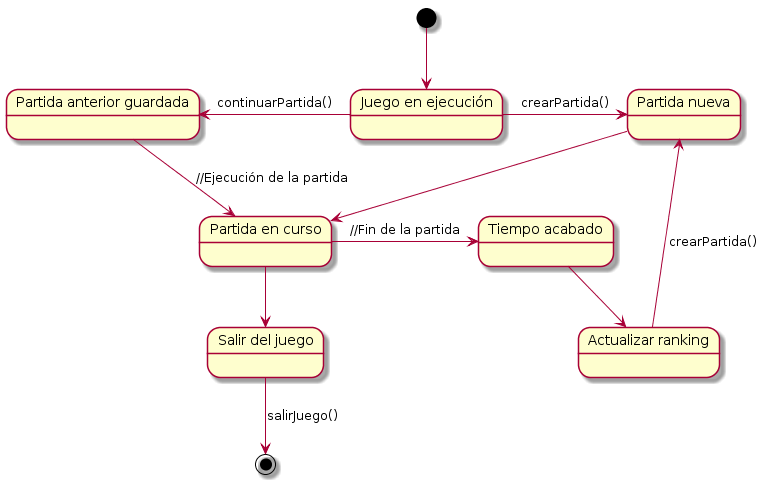
\includegraphics[width=0.9\textwidth]{./imatges/Estados_juego.png}
  \end{center}
  Tenemos que es estado inicial de este diagrama es Juego en ejecución, una vez estamos en este estado tenemos dos opciones, continuar una partida ya existente (partida guardada) o bien, empezar una partida nueva. En ambas situaciones, el proximo estado, es la ejecución de la partida.
  \\A continuación se pueden dar dos casos, uno de ellos es que se haya acabado el tiempo, y por lo tanto la partida finaliza, posteriormente, se pasa a actualizar el ranking, y se empieza una partida nueva.
  \\El segundo caso es que sea el jugador quien desee terminar la partida, en esta situación simplemente se sale del juego, y llegamos al estado final.